\documentclass[conference]{IEEEtran}
\IEEEoverridecommandlockouts
% The preceding line is only needed to identify funding in the first footnote. If that is unneeded, please comment it out.
\usepackage{cite}
\usepackage{amsmath,amssymb,amsfonts}
\usepackage{algorithmic}
\usepackage{graphicx}
\usepackage{textcomp}
\usepackage{xcolor}
\def\BibTeX{{\rm B\kern-.05em{\sc i\kern-.025em b}\kern-.08em
    T\kern-.1667em\lower.7ex\hbox{E}\kern-.125emX}}
\begin{document}

\title{Network Security Lab 1: Packet Tracer – Configuring RIPv2}

\author{\IEEEauthorblockN{Alexander Hoffmann}
\IEEEauthorblockA{\textit{ECE Paris}\\
Paris, France \\
alexander.hoffmann@edu.ece.fr}
}

\maketitle

\section{Configure RIPv2}

\subsection{Configure RIPv2 on R1}

\textbf{a.} We configure a static IP route using the \texttt{ip route} command followed by the IP address and the interface.
\begin{verbatim}
# ip route 0.0.0.0 0.0.0.0 S0/0/1
\end{verbatim}
The internet traffic is now routed towards the cloud. We print the ip routes which yields the following results:
\begin{center}
\begin{figure}[h]
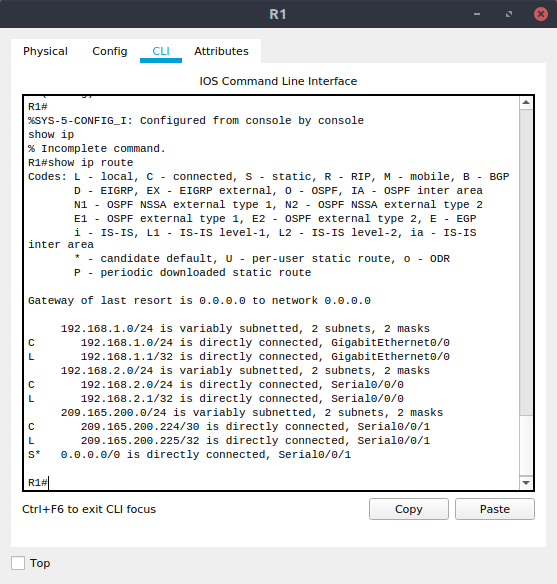
\includegraphics[scale=0.45]{../q01a.png}
\caption{IP routes}
\end{figure}
\end{center}

\textbf{b.} To enter RIP protocol configuration mode, use the following command:
\begin{verbatim}
# router rip
\end{verbatim}
\begin{center}
\begin{figure}[h]
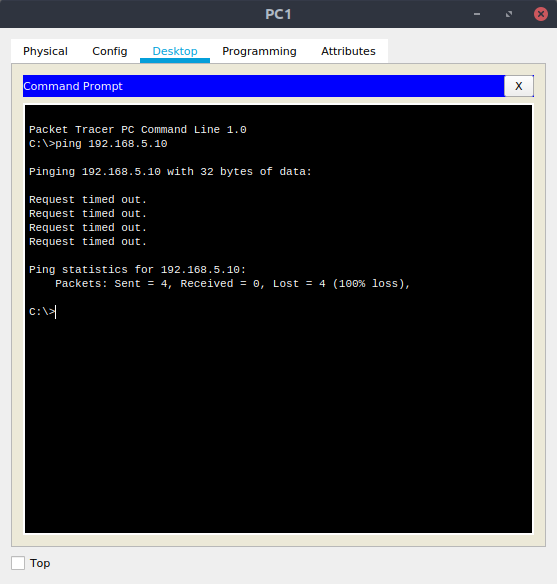
\includegraphics[scale=0.45]{../q01b.png}\
\caption{Ping PC3 from PC1}
\end{figure}
\end{center}

\textbf{c.} We want to use version 2 of the RIP protocol, which is done with the following command:
\begin{verbatim}
# version 2
# no auto-summary
\end{verbatim}

\textbf{d.} Configure RIP for the networks that connect to R1.
\begin{verbatim}
# 192.168.1.0
# 192.168.2.0
\end{verbatim}

\textbf{e.} Configure the LAN port that contains no routers so that it does not send out any routing information.
\begin{verbatim}
# passive-interface gig 0/0
\end{verbatim}

\textbf{f.} Advertise the default route configured in step 1a with other RIP routers.
\begin{verbatim}
# default-information originate
\end{verbatim}

\textbf{g.} Change the configuration.
\begin{verbatim}
# copy running-config startup-config
\end{verbatim}
\begin{center}
\begin{figure}[h]
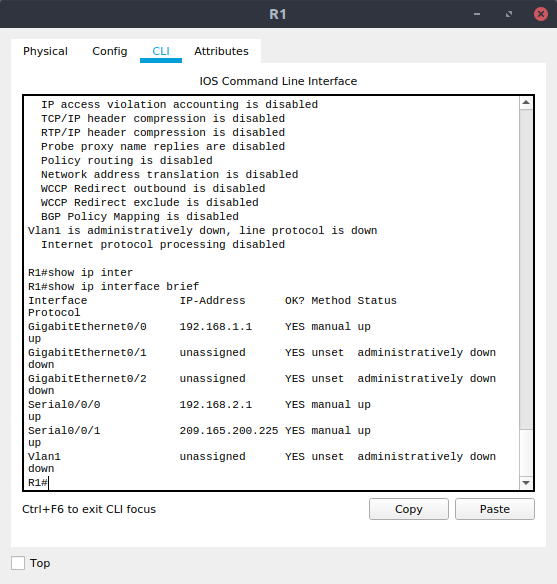
\includegraphics[scale=0.45]{../q01g.png}
\caption{IP interfaces}
\end{figure}
\end{center}

\subsection{Configure RIPv2 on R2}

\textbf{a.} Enter RIP protocol configuration mode.
\begin{verbatim}
# router rip
\end{verbatim}

\textbf{b.} We want to use version 2 of the RIP protocol, which is done with the following command:
\begin{verbatim}
# version 2
# no auto-summary
\end{verbatim}

\textbf{c.} Configure RIP for the networks directly connected to R2.
\begin{verbatim}
# network 192.168.2.0
# network 192.168.3.0
# network 192.168.4.0
\end{verbatim}

\textbf{d.} Configure the interface that contains no routers so that it does not send out routing information.
\begin{verbatim}
# passive-interface gig0/0
\end{verbatim}

\textbf{g.} Change the configuration.
\begin{verbatim}
# copy running-config startup-config
\end{verbatim}

\subsection{Configure RIPv2 on R3}

\begin{verbatim}
# router rip
# version 2
# no auto-summary
# network 192.168.4.0
# network 192.168.5.0
# passive-interface gig0/0
\end{verbatim}

\section{Verify configurations}

\subsection{View routing tables of R1, R2 and R3}

\textbf{a.}
\begin{center}
\begin{figure}[h]
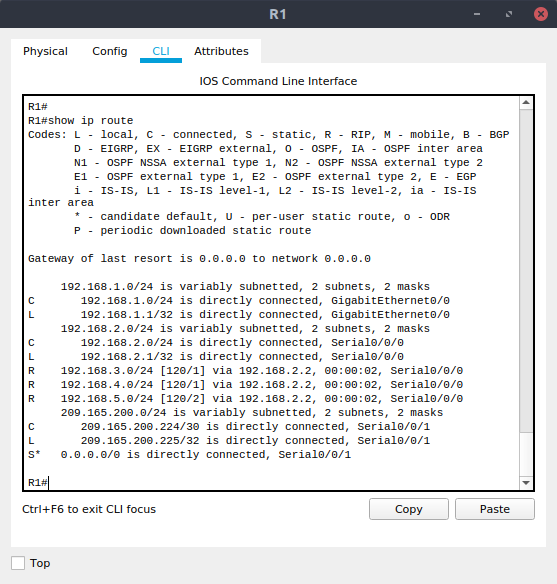
\includegraphics[scale=0.45]{../q02a.png}
\caption{IP routes}
\end{figure}
\end{center}

\textbf{b.}
\begin{center}
\begin{figure}[h]
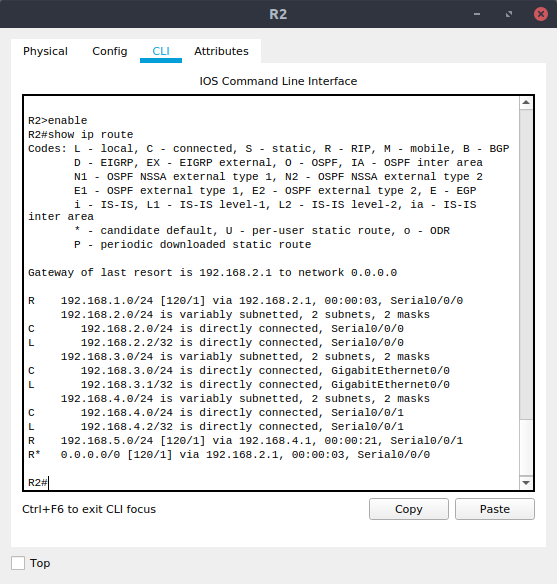
\includegraphics[scale=0.45]{../q02b1.png}
\caption{IP routes}
\end{figure}
\begin{figure}[h]
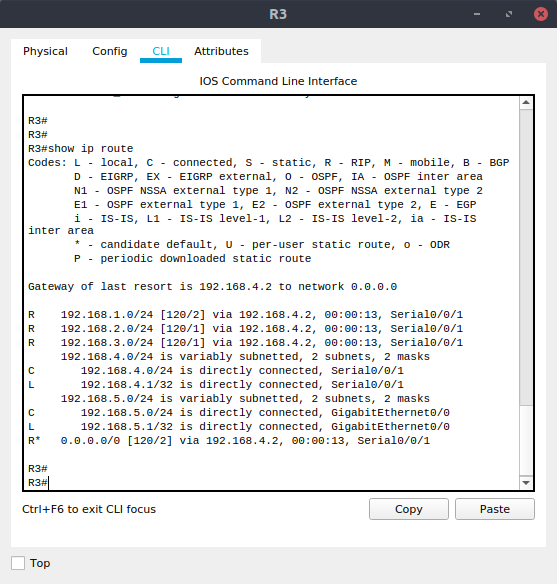
\includegraphics[scale=0.45]{../q02b2.png}
\caption{IP routes}
\end{figure}
\end{center}

\subsection{Verify full connectivity to all destinations}
We can ping the server from every PC.
\begin{center}
\begin{figure}[h]
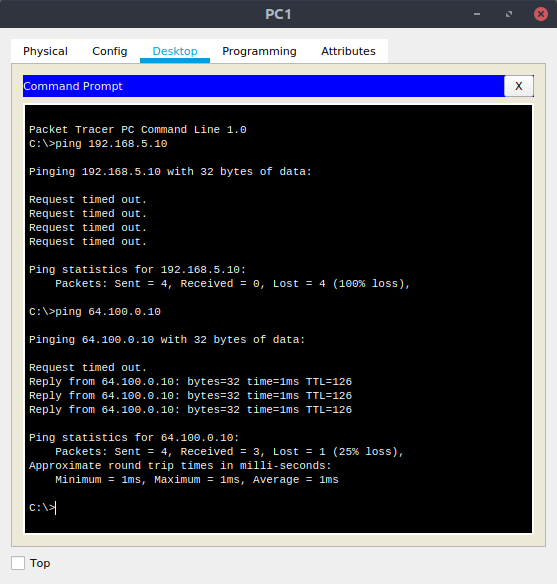
\includegraphics[scale=0.45]{../q03a.png}
\caption{PC1 can ping Server}
\end{figure}
\begin{figure}[h]
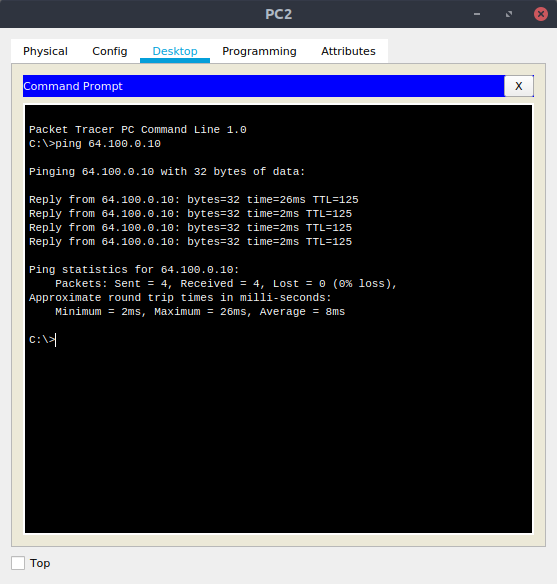
\includegraphics[scale=0.45]{../q03b.png}
\caption{PC2 can ping Server}
\end{figure}
\begin{figure}[h]
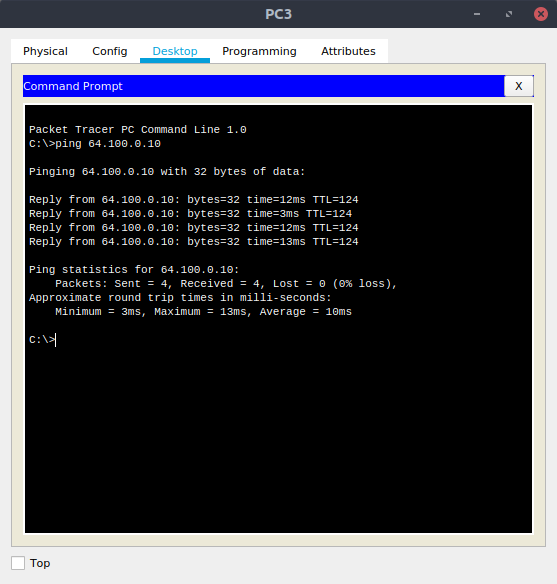
\includegraphics[scale=0.45]{../q03c.png}
\caption{PC3 can ping Server}
\end{figure}
\end{center}

\end{document}
